\documentclass[10pt]{article}
%	options include 12pt or 11pt or 10pt
%	classes include article, report, book, letter, thesis

\usepackage[a4paper,bindingoffset=0.2in,%
left=1in,right=1in,top=0.2in,bottom=0.3in,%
footskip=.15in]{geometry}

\usepackage[T1]{fontenc}
\usepackage[polish]{babel}
\usepackage[utf8]{inputenc}
\usepackage{lmodern}
\usepackage{pgfplots}
\usepackage{graphicx}
\usepackage{amsmath}
\usepackage{subcaption}
\usepackage{multirow}
\newtheorem{hip}{Hipoteza}
\newtheorem{que}{Pytanie}
\newtheorem{wn}{Wniosek}
\newtheorem{wyd}{Zadanie}

\title{Algorytmy numeryczne}
\author{Zadanie 2 \\ Dawid Bińkuś \& Oskar Bir \& Mateusz Małecki\\grupa 1 tester-programista}
\date{11 Listopad 2018}

\begin{document}
\maketitle 

\section{Operacje na macierzach}
Sprawozdanie prezentuje analizę wydajności i poprawności implementacji algorytmu eliminacji Gaussa, dla losowej macierzy kwadratowej $A$ i wektora $B$ w układzie liniowym
$A\cdot X = B.$\\
Zaimplementowano następujące warianty algorytmu:
\begin{itemize}
	\item[G:]bez wyboru elementu podstawowego,
	\item [PG:]z częściowym wyborem elementu podstawowego,
	\item [FG:]z peanym wyborem elementu podstawowego.
\end{itemize}
Dodatkowo, obliczenia zostały wykonane, używając trzech różny typów reprezentujących liczbę rzeczywistą:
\begin{itemize}
	\item[TF:]typ pojedynczej precyzji: \textbf{float}
	\item[TD:]typ podwójnej precyzji: \textbf{double}
	\item[TC:]własna implementacja, przechowująca liczbę w postaci ułamka liczb całkowitych: \textbf{fraction}
\end{itemize}
$\text{Jako współczynniki macierzy } A \text{ oraz wektora } X \text{ zostały wylosowane liczby zmiennoprzecinkowe z przedziału: }$\\
$[\frac{-2^{16}}{2^{16}},\frac{2^{16}-1}{2^{16}}]$ Następnie wektor $B$ został wyliczony wedługo wzoru $B = A\cdot X$.
Macierz $A$ i wektor $B$ zostają podane jako parametry do rozwiązania układu równań, wektor $X$ zaś pozostawiamy jako rozwiązanie wzorcowe, za pomocą którego obliczamy błąd wykonanego algorytmu.\\\\
Program do realizacji testów został wykonany w języku \textit{Java}. Typ danych \textit{TC} został zaimplementowany za pomocą wbudowanego typu całkowitego \emph{BigInteger}. Testy zostały wykonane na macierzach o rozmiarze $\{10,20,...,500\}$ (float,double) $\{10,20...,150\}$ (fraction) 
w ilości prób malejącej, wraz z wykonywaniem testów na coraz to większych macierzach. Wyniki zostały zagregowane za pomocą średniej arytmetycznej.
\section{Analiza hipotez}
Rozważmy następujące wykresy (Rysunek\ref{rys})
\begin{figure}[h]
	\caption{Wykresy reprezentujące błąd bezwzględny oraz czas wykonania dla różnych typów danych oraz różnych wariantów algorytmu\label{rys}}
	\begin{subfigure}{0.5\textwidth}
		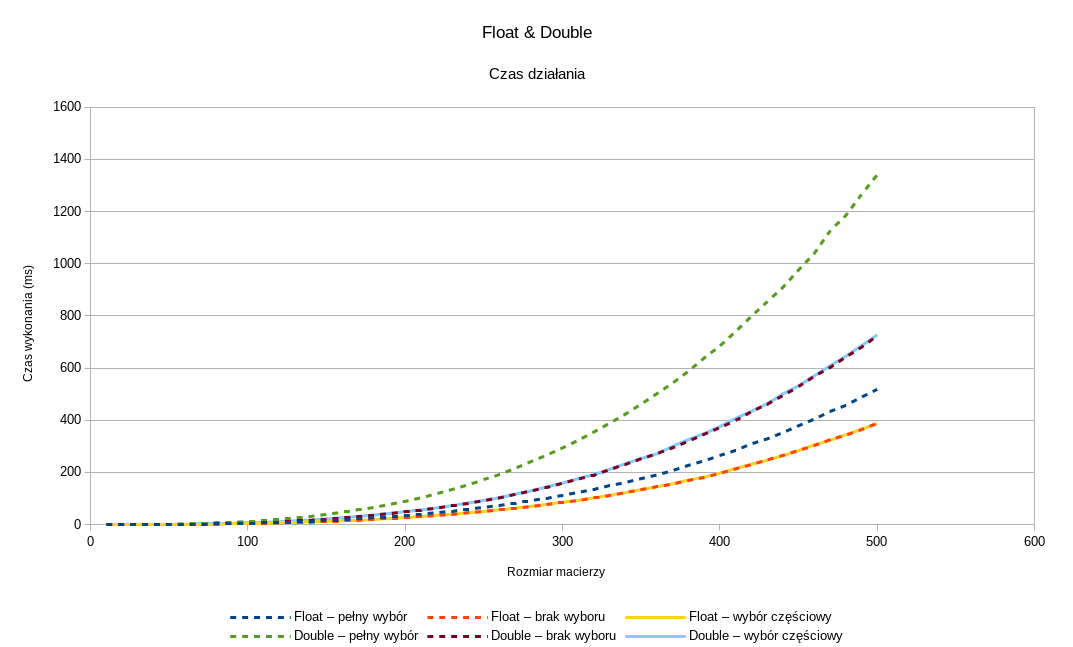
\includegraphics[width=\textwidth]{float_double_czas.png}
		\caption{ \label{Rys1a}}
	\end{subfigure}
	\hfill
	\begin{subfigure}{0.5\textwidth}
		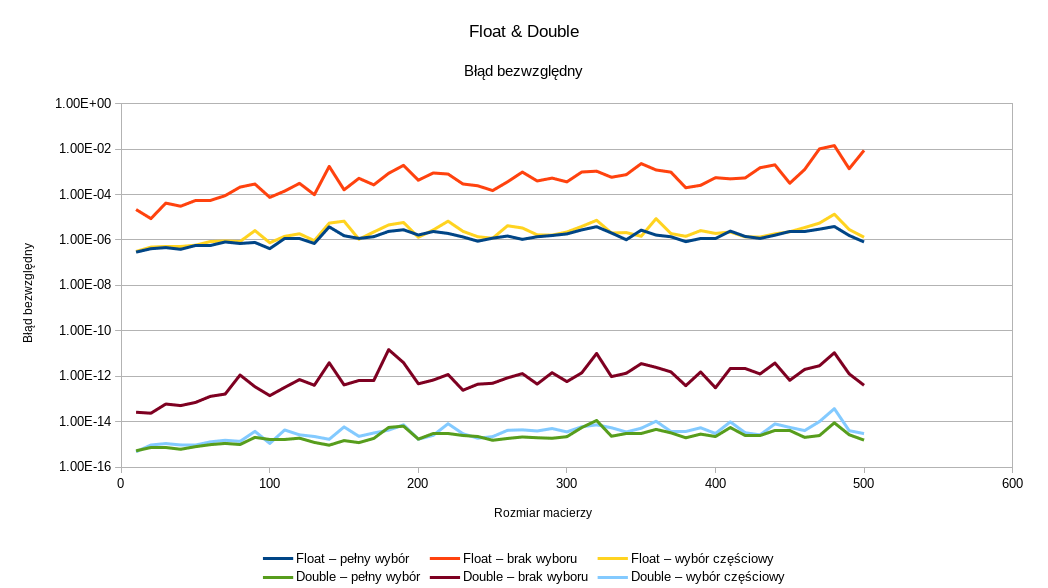
\includegraphics[width=\textwidth]{float_double_blad.png}
		\caption{  \label{Rys1b}}
	\end{subfigure}
	
	\begin{subfigure}{0.5\textwidth}
		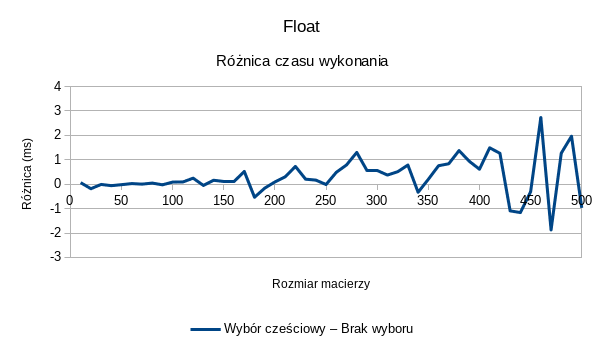
\includegraphics[width=\textwidth]{float_roznica_czas.png}
		\caption{ \label{Rys1c}}
	\end{subfigure}
	\hfill
	\begin{subfigure}{0.5\textwidth}
		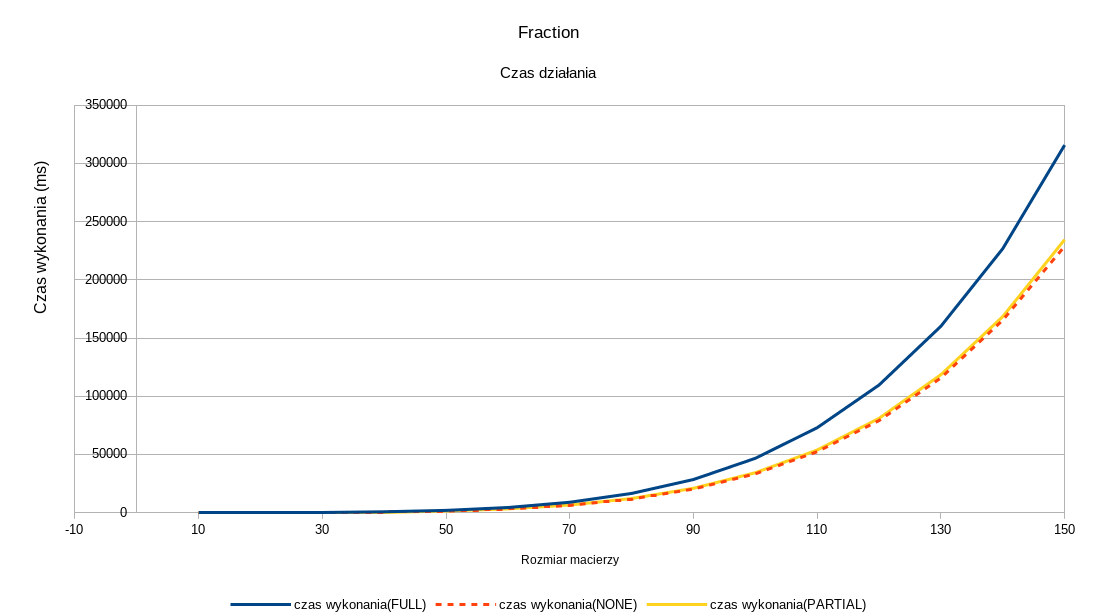
\includegraphics[width=\textwidth]{fraction_czas.png}
		\caption{ \label{Rys1d}}
	\end{subfigure}
	\begin{tabular}{ |l|l|l|l|l|l|l|l|l|l| }
	\hline
	\multicolumn{10}{ |c| }{Fractial - porównanie} \\
	n & \multicolumn{3}{|c|}{Błąd bezwzględny} & \multicolumn{3}{|c|}{Czas wykonania} & \multicolumn{3}{|c|}{Ilość prób}\\
	\hline
	Wariant -> & G & PG & FG & G & PG & FG & \multicolumn{3}{|c|}{}\\
	\hline
	10 & 0 & 0 & 0 & 2.39034797 & 2.70733242 & 2.62618003 & \multicolumn{3}{|c|}{100} \\
	20 & 0 & 0 & 0 & 26.08455804 & 28.1878754 & 37.95241776 &\multicolumn{3}{|c|}{25} \\
	50 & 0 & 0 & 0 & 1353.7187555 & 1418.31329225 & 1935.74870875 & \multicolumn{3}{|c|}{4} \\
	100 & 0 & 0 & 0 & 33360.40558 & 34285.387315 & 46668.033684 & \multicolumn{3}{|c|}{1} \\
	130 & 0 & 0 & 0 & 115763.860973 & 118493.372512 & 160113.679247 & \multicolumn{3}{|c|}{1} \\
	150 & 0 & 0 & 0 & 228794.993101 & 234503.568338 &  315739.697225 & \multicolumn{3}{|c|}{1} \\
	\hline
\end{tabular}
\caption{Tabela prezentująca porównanie wyników dla typu Fractial}
\label{tab:1}
\end{figure}
Prezentują one błąd bezwzględny wartości w skali logarytmicznej (chyba że jest podane inaczej), wyliczonej za pomocą wcześniej wspomnianych algorytmów wobec wektora wzorcowego $X$.\\
Część z nich prezentuje również czas wykonania algorytmu podany w milisekundach.
\subsection{Związek czasu wykonywania z wariantem algorytmu eliminacji Gaussa}
\begin{hip}
	Dla dowolnego ustalone rozmiaru macierzy czas działania metody Gaussa w kolejnych wersjach (G,PG,FG) rośnie.\label{hip:1}
\end{hip}
Przeanalizujmy wykresy \ref{Rys1a} oraz \ref{Rys1d}. Zaprezentowano na nich porównanie czasu wykonania w zależności od wybranego typu danych oraz wariantu algorytmu. Niezależnie od typu danych można zauważyć pewną tendencję.\\
Po pierwsze, wraz z wzrostem rozmiaru macierzy użytej do rozwiązania układu równań, można zauważyć znaczący wzrost czasu wykonywania dla wariantu FG względem wariantów G i PG. Wykonując operacje na małych macierzach proces rozwiązywania nie jest na tyle skomplikowany by w jakikolwiek sposób wpływać na wydajność.
Drugą interesującą rzeczą natomiast jest, brak znaczących różnic między wariantem G i PG. By bardziej uwidocznić to zjawisko przeanalizujmy wykres \ref{Rys1c}, który prezentuje różnicę między cześciowym wyborem elementu podstawowego a brakiem wyboru w przypadku typu danych float. Wynikają z niego dwie rzeczy: różnica między wykonywaniem tych dwóch argumentów jest praktycznie nieznacząca (zaledwie kilka milisekund). Drugą rzeczą jest natomiast fakt, że wariant PG zdaje się być nieznacznie wolniejszy od wariantu G (Wraz z wzrostem rozmiaru macierzy okazuje sie w niektorych wypadkach nawet wydajniejszy niz standardowy algorytm Gaussa)
\begin{wn}
	Hipoteza okazuje się być cześciowo prawidziwa. Wariant FG powoduje znaczny wzrost czasu wykonania dla wszystkich wykorzystanych typów danych. Interesujący natomiast jest brak znaczących różnic między wariantami PG i G, który jest spowodowany niewielkim wpływem na czas wykonania (w wariancie PG sprawdzamy tylko $n$ wartości w przeciwieństwie do $n*n$ w wariancie FG).\label{wn:1}
\end{wn}
\subsection{Związek błędu obliczeń z wariantem algorytmu eliminacji Gaussa}
\begin{hip}
	Dla dowolnego ustalonego rozmiaru macierzy błąd uzyskanego wyniku metody Gaussa w kolejnych wersjach (G,PG,FG) maleje.\label{hip:2}
\end{hip}
Przeanalizujmy wykres \ref{Rys1b}. Prezentuje on zestawienie błędu bezwzględnego rozwiązania układu równań względem wektora $X$ dla typów danych float i double. W przypadku obu typów danych najmniej dokładny jest wariant G (różnice między nimi są efektem zastosowanej precyzji w tych typach). W przypadku wariantów PG i FG można zauważyć iż mają one bardzo zbliżoną dokładność z małą przewagą wariantu PG - jego dodatkowym atutem jest większa stabliność wyników. W sytuacjach gdy wariant G i PG mają problemy z bardziej skomplikowanymi równaniami (charakterystyczne wzrosty na wykresie) - PG radzi sobie zdecydowanie lepiej.
\begin{wn}
	Hipoteza okazuje się być prawdziwa. Wariant PG zapewnia największą dokładność i stabilność wyników względem nieco gorszego FG oraz G, w którym różnica błędu sięga nawet dwóch rzędów wielkości. Jednakże biorąc pod uwagę \ref{wn:1} najbardziej opłacalnym w kategorii dokładność/wydajność okazuje się być wariant PG jako iż różnice błędu między nim a pełnym wyborem zdają się być akceptowalne gdy weźmiemy pod uwagę znacznie szybszy czas działania.\label{wn:2}
\end{wn}
\subsection{Poprawność własnej arytmetyki}
\begin{hip}
	Użycie własnej arytmetyki na ułamkach zapewnia bezbłędne wyniki niezależnie od wariantu metody Gaussa i rozmiaru macierzy.\label{hip:3}
\end{hip}
Przeanalizujmy tabelę \ref{tab:1}\\
Prezentuje ona wyniki z użyciem własnej arytmetyki dla wszystkich wariantów algorytmu.
Obliczenia zostały wykonane na macierzach o rozmiarze $n$ w przedziale $\{10,20,...,150\}$ z racji ograniczeń sprzętowych. Rozpatrując wyniki testów, można dość do wniosku, że użycie własnej artymetyki całkowicie eliminuje błąd obliczeń. Jest to spowodowane charakterystyką typu BigInteger. Teoretycznie, typ ten nie ma żadnego limitu przechowywanych danych - w zależności od potrzeb zajmuje potrzebną ilość pamięci w komputerze. Jedynym ogranicznikiem w przypadku typu BigInteger jest pamięć naszego komputera. Dodając do tego sposób przechowywania ułamków ($\frac{licznik}{mianownik}$) jesteśmy w stanie wykonywać bardzo skomplikowane równania bez utraty precyzji.
\begin{wn}
	Hipoteza 3 okazuje się być prawdziwa. Użycie własnej arytmetyki zapewnia teoretycznie największą możliwą dokładność przechowywanych danych w porównaniu do zwykłych typów zmiennoprzecinkowych. Dzięki temu, wszelkie operacje wykonywane na typie Fraction są wykonywane z dokładnością równą 0\label{wn:3}
\end{wn}
\section{Pytania}
\begin{figure}[h]
	\caption{Wykresy reprezentujące błąd bezwzględny dla różnych sposobów sumowania}
	\begin{subfigure}{0.5\textwidth}
		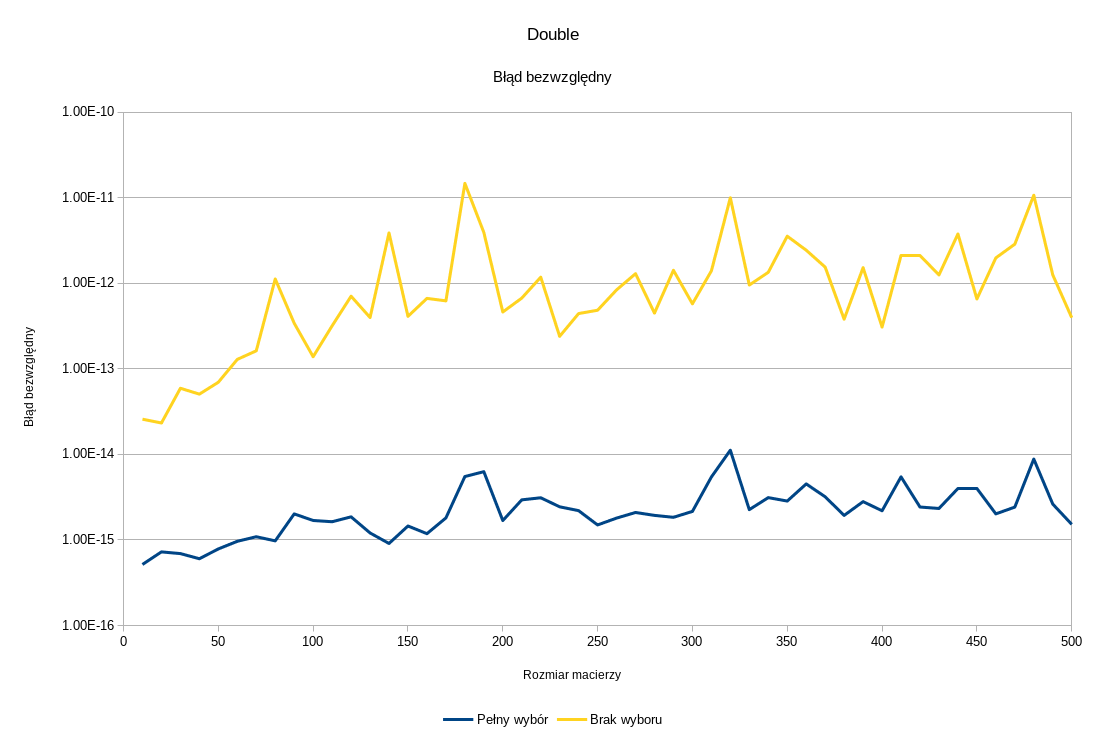
\includegraphics[width=\textwidth]{double_full_none_blad.png}
		\caption{ \label{Rys2a}}
	\end{subfigure}
	\hfill
	\begin{subfigure}{0.5\textwidth}
		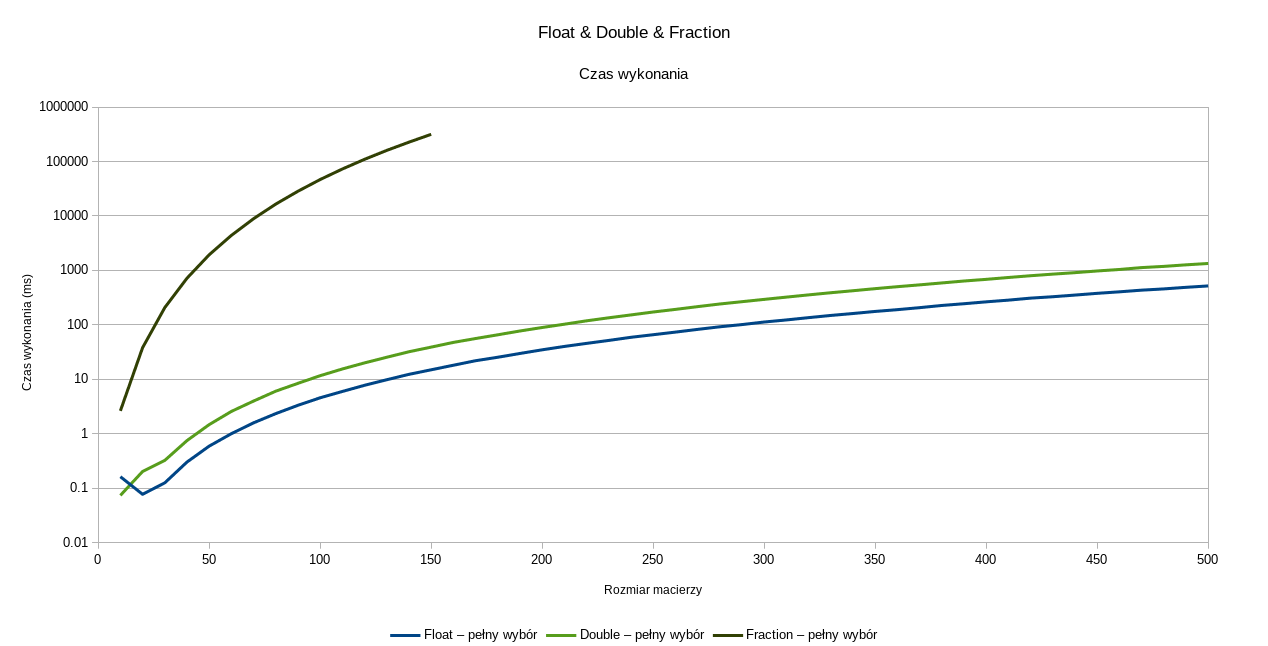
\includegraphics[width=\textwidth]{float_double_fract_full_czas.png}
		\caption{  \label{Rys2b}}
	\end{subfigure}
\end{figure}
\subsection{Dokładność obliczeń (typ podwójnej precyzji)}
\begin{que}
	Jak zależy dokładnośc obliczeń (błąd) od rozmiaru macierzy dla dwóch wybranych
	przez Ciebie wariantów metody Gaussa gdy obliczenia prowadzone są na typie
	podwójnej precyzji (TD)?\label{que:1}
\end{que}
\subsection{Zależność czasu działania algorytmu od rozmiaru macierzy oraz typu}
\begin{que}
	 Jak przy wybranym przez Ciebie wariancie metody Gaussa zależy czas działania
	algorytmu od rozmiaru macierzy i różnych typów?\label{que:2}
\end{que}
\section{Wydajność implementacji}
\begin{wyd}
	Podaj czasy rozwiązania układu równań uzyskane dla macierzy o rozmiarze $500$ dla $9$ testowanych wariantów.
\end{wyd}
\section{Podział pracy}
\begin{center}
	\begin{tabular}{| l | l | l |}
		\hline
		\textbf{Dawid Bińkuś} & \textbf{Oskar Bir} & \textbf{Mateusz Małecki} \\ \hline
		Struktura projektu & Ten też coś robił & A ten to w ogóle bardzo dużo \\ \hline
		Przygotowanie sprawozdania & Coś & Coś\\ \hline
		Implementacja algorytmu Gaussa w wariantach PG i FG & Coś & Coś \\ \hline
		
		
	\end{tabular}
\end{center}
\end{document}